\documentclass[conference]{IEEEtran}
\IEEEoverridecommandlockouts
% The preceding line is only needed to identify funding in the first footnote. If that is unneeded, please comment it out.
\usepackage{cite}
\usepackage{amsmath,amssymb,amsfonts}
\usepackage{algorithmic}
\usepackage{graphicx}
\usepackage{textcomp}
\usepackage{xcolor}
\usepackage{hyperref}
\usepackage{enumitem}
\usepackage{ulem}
\def\BibTeX{{\rm B\kern-.05em{\sc i\kern-.025em b}\kern-.08em
    T\kern-.1667em\lower.7ex\hbox{E}\kern-.125emX}}
\begin{document}

\title{Tutorial: Markov Chain Monte Carlo Methods for Various Optimization Problems*\\
{\footnotesize \textsuperscript{*}For ECE 506 project, Fall 2018}
\thanks{}
}

\author{\IEEEauthorblockN{Mustafa S Salman}
\IEEEauthorblockA{\textit{Dept. of Electrical \& Computer Engineering} \\
\textit{University of New Mexico}\\
Albuquerque, NM, USA \\
esalman@unm.edu}
}

\maketitle

\begin{abstract}
There are several well-known and tested methods for optimization of differentiable and deterministic problems, including but not limited to the gradient descent, BFGS and Newton's methods and their variants. On the other hand, Markov Chain Monte Carlo methods are useful for solution of non-differentiable and non-deterministic problems. The goal of this project is to study and compare the performance of Markov Chain Monte Carlo methods for various deterministic and non-deterministic optimization NP-hard problems.
\end{abstract}

\begin{IEEEkeywords}
optimization, gradient descent, BFGS, Newton's method, Markov Chain Monte Carlo, MCMC
\end{IEEEkeywords}

\section{Motivation}
In many circumstances, mathematical models of physical systems becomes so complex that inverse methods cannot be used to compute the model parameters. Markov-chain Monte Carlo (MCMC) methods are simple numerical approaches appropriate for this type of situations. MCMC method can be used to determine an optimal parameter set for a model of arbitrary complexity by minimizing a cost function \cite{b6}. It does not require the estimation of the gradient of the goodness-of-fit function, thus has an advantage over gradient descent methods \cite{b7} in optimizing non-differentiable functions. There exists non-deterministic optimization problems with many local optima and complicated constraints, and a possible mix of continuous and discrete variables. MCMC is at the core of randomized optimization methods such as stochastic approximation, simulated annealing, evolutionary algorithms and cross-entropy methods which can be used to solve both random and deterministic problems \cite{b8}. Therefore I am interested in studying MCMC methods.

\section{Expected Contribution}

\begin{enumerate}
	\item{Implementing deterministic algorithm(s) (steepest descent, BFGS, Newton's method etc.) in Python}
	\item{Implementing randomized optimization algorithm(s) (stochastic approximation, \sout{simulated annealing}, evolutionary algorithm, cross-entropy method etc.) in Python}
	\item{Using randomized optimization algorithm(s) to solve deterministic problem(s) and compare the validation metrics with the deterministic algorithm(s)}
	\item{Using randomized optimization algorithm(s) to solve NP-hard problem(s) and (if possible) compare with the deterministic algorithms}
\end{enumerate}

Fig. \ref{fig} shows a summary of the types of probelems and algorithms which may be covered in this project.

\begin{figure}[tbp]
\centerline{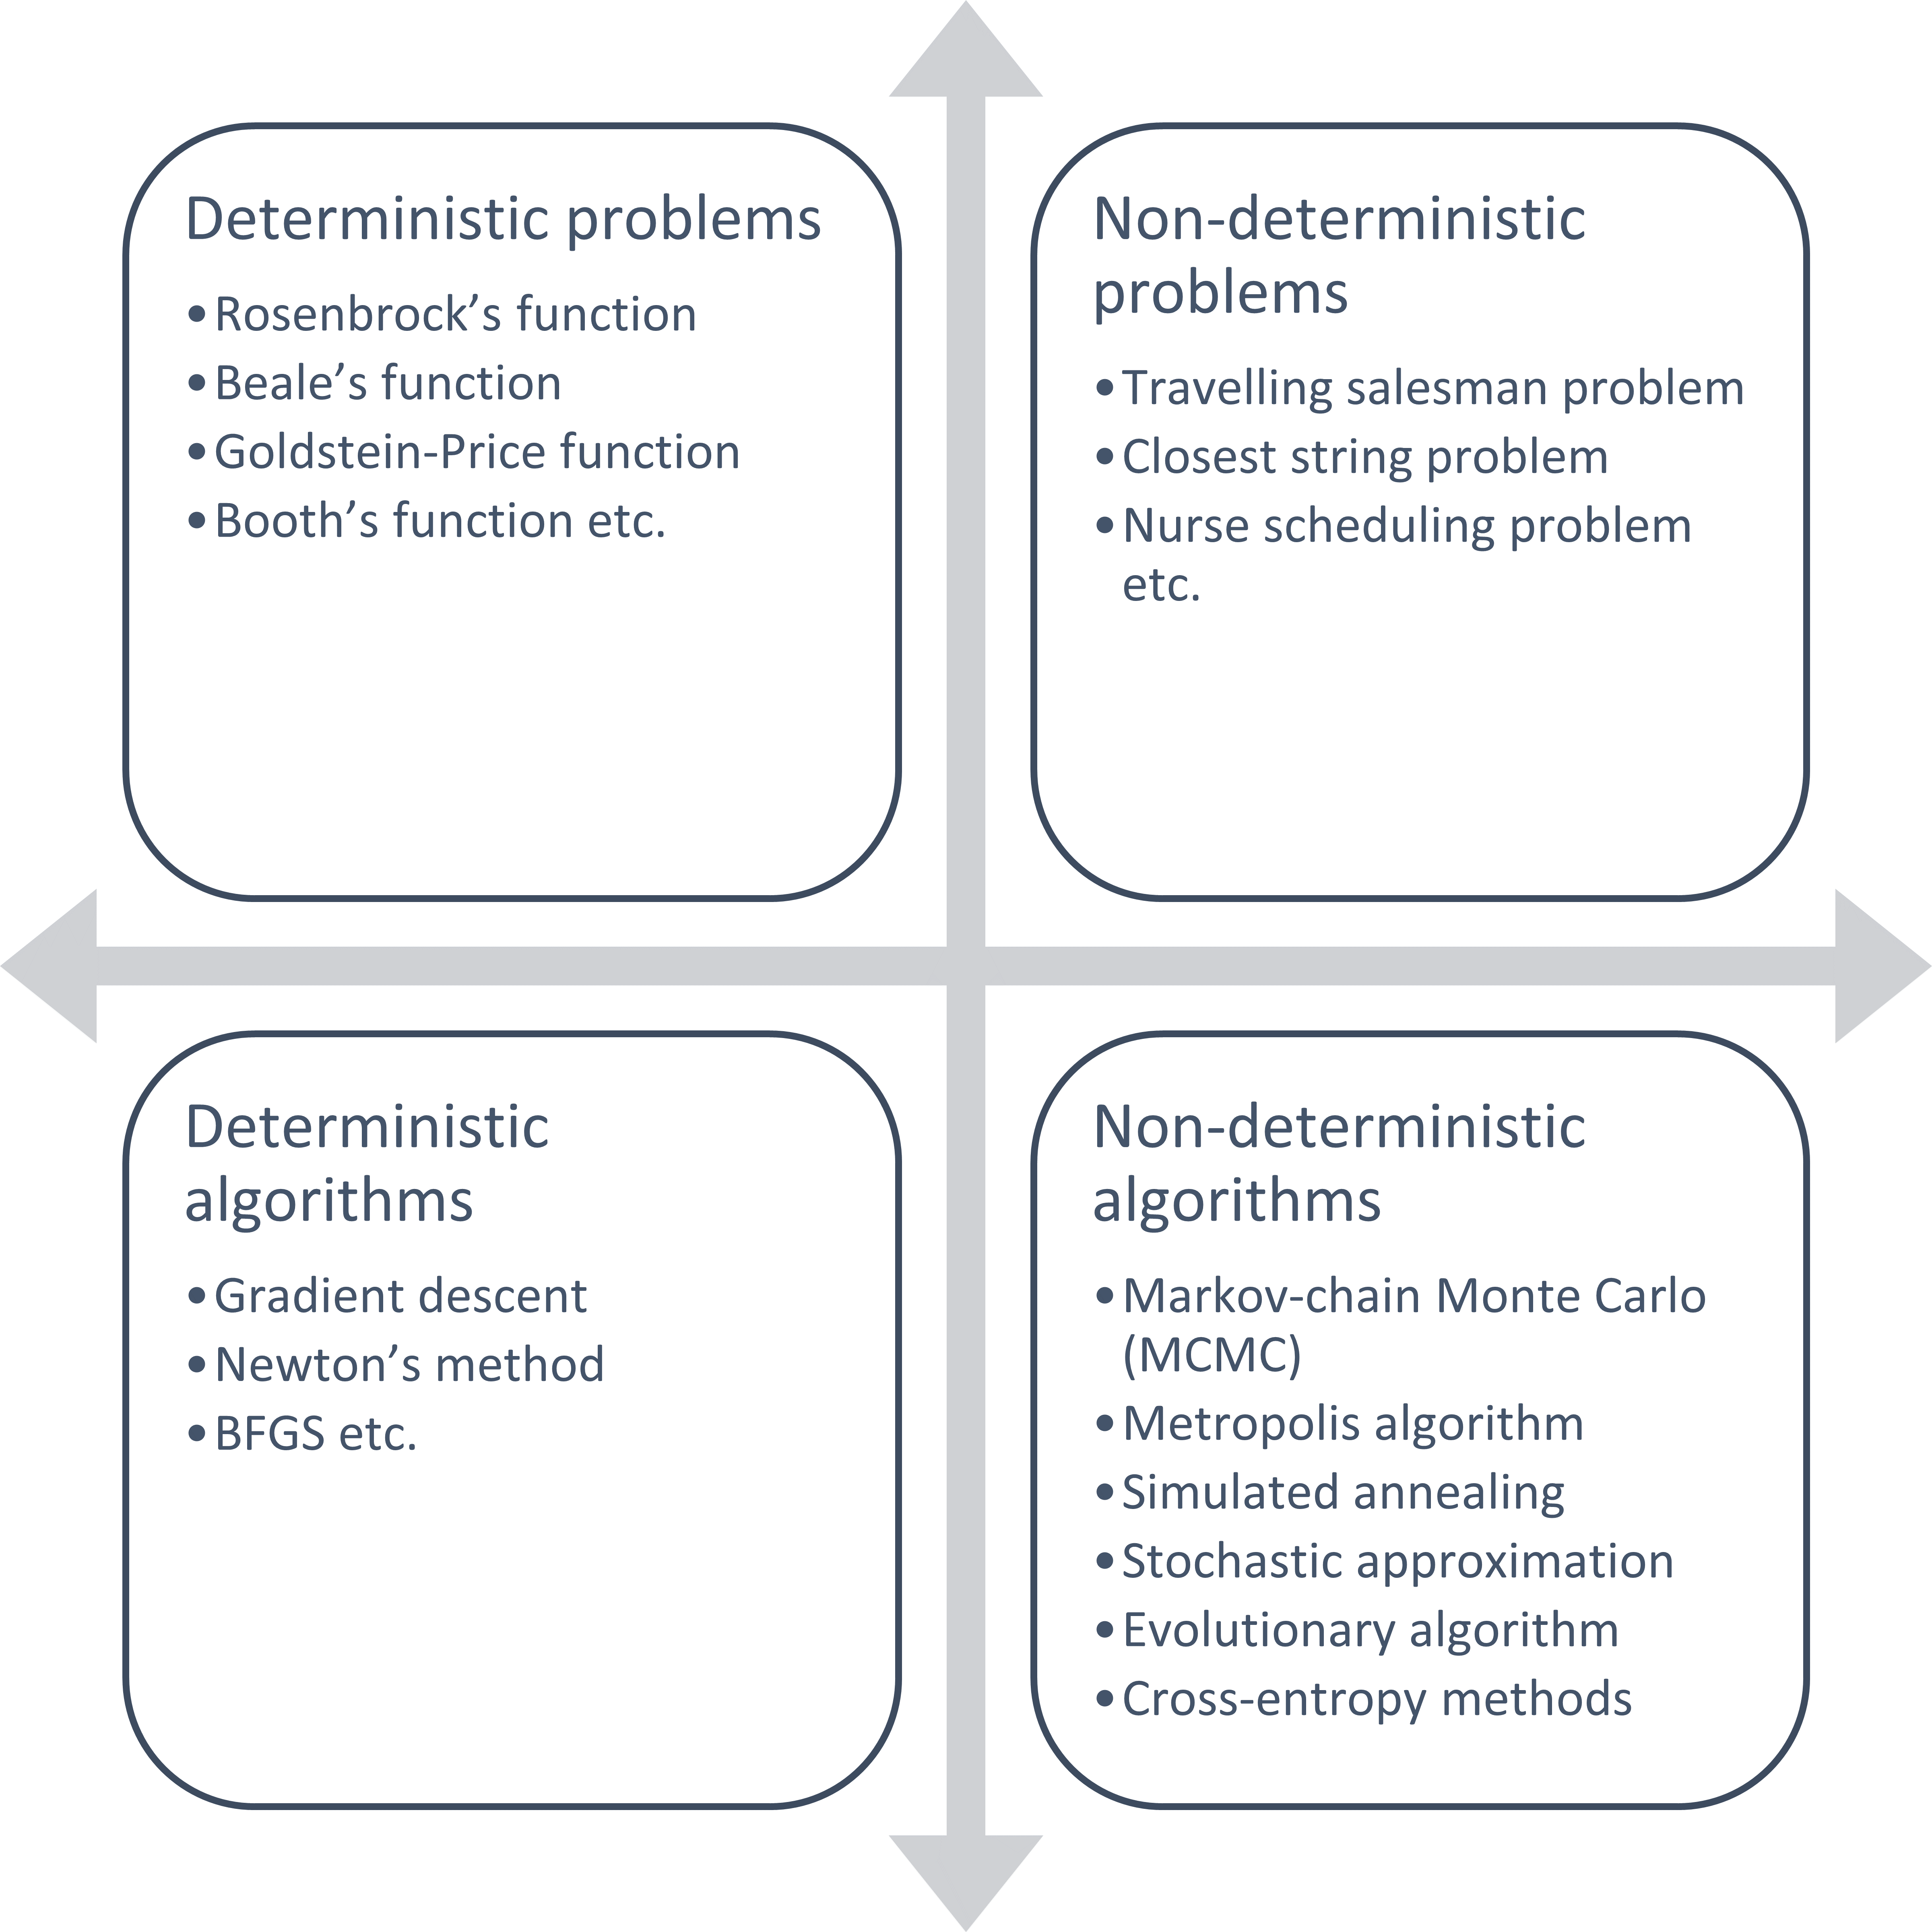
\includegraphics[width=85mm]{flowchart.png}}
\caption{Various types of optimization problems and algorithms}
\label{fig}
\end{figure}

% \begin{table}[htbp]
% \caption{Expected contributions}
% \begin{center}
% \begin{tabular}{|c|c|}
% \hline
% \textbf{Table}&\multicolumn{3}{|c|}{\textbf{Table Column Head}} \\
% \cline{2-4} 
% \textbf{Head} & \textbf{\textit{Table column subhead}}& \textbf{\textit{Subhead}}& \textbf{\textit{Subhead}} \\
% \hline
% copy& More table copy$^{\mathrm{a}}$& &  \\
% \hline
% \multicolumn{4}{l}{$^{\mathrm{a}}$Sample of a Table footnote.}
% \end{tabular}
% \label{tab1}
% \end{center}
% \end{table}

\begin{figure*}[tbp]
\centerline{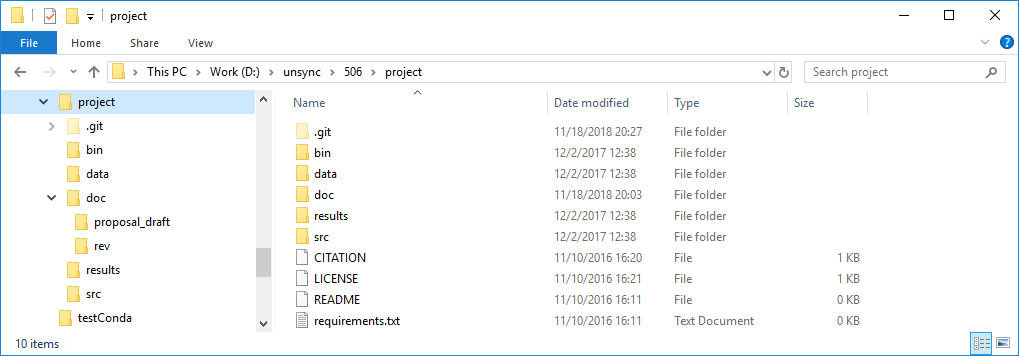
\includegraphics[width=130mm]{../../results/Capture.PNG}}
\caption{Project template directory}
\label{fig1}
\end{figure*}

\section{Code}
I intend to use Python for this project. Fig. \ref{fig1} shows a screenshot of the project template folder. Following is the description of the contents of the template folder:

\begin{description}[style=multiline,leftmargin=6em]
	\item[\textbf{.git}]{contains Git versioning information.}
	\item[\textbf{bin}] contains libraries and packages required to run the project.
	\item[\textbf{data}] contains unprocessed data acquired for using in the project.
	\item[\textbf{doc}] contains all the documentations (revision, project proposal etc.), including the \LaTeX sources. I have chosen \LaTeX over Microsoft Word which is difficult to maintain. Although Jupyter Notebook would be a great tool for maintaining the source code and documentation, it is difficult for version control and I also intend to write the project proposal and other documents in the IEEE format instead of in a Jupyter Notebook.
	\item[\textbf{results}] contains processed data and any other output from running the source code, including figures.
	\item[\textbf{src}] contains the source codes.
	\item[\textbf{CITATION}] contains the information about how to cite this project.
	\item[\textbf{README}] brief project README document.
	\item[\textbf{LICENSE}] contains copyright and licensing information of the project.
	\item[\textbf{req...s.txt}] required for automatic deployment.
\end{description}

\section{Data}
For this project I have searched for problems/functions to optimize. Here I am listing some problems that I have found which might be worth investigating for the use of the algorithms.

\subsection{Differentiable/Deterministic Problems}
This classes of functions will be obtained from Wikipedia \cite{b3}. Some examples are shown in Fig. \ref{testfunfig}

\begin{figure}[tbp]
\begin{tabular}{cc}
  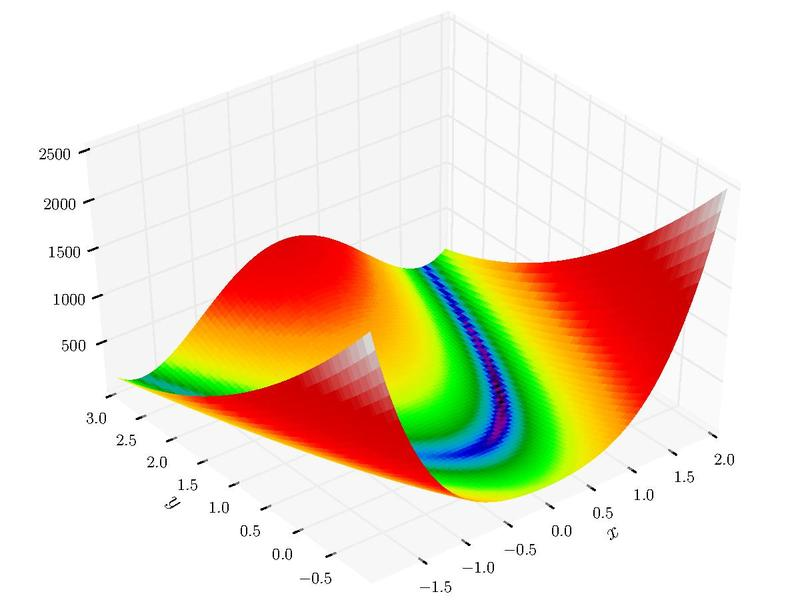
\includegraphics[width=35mm]{Rosenbrock} &   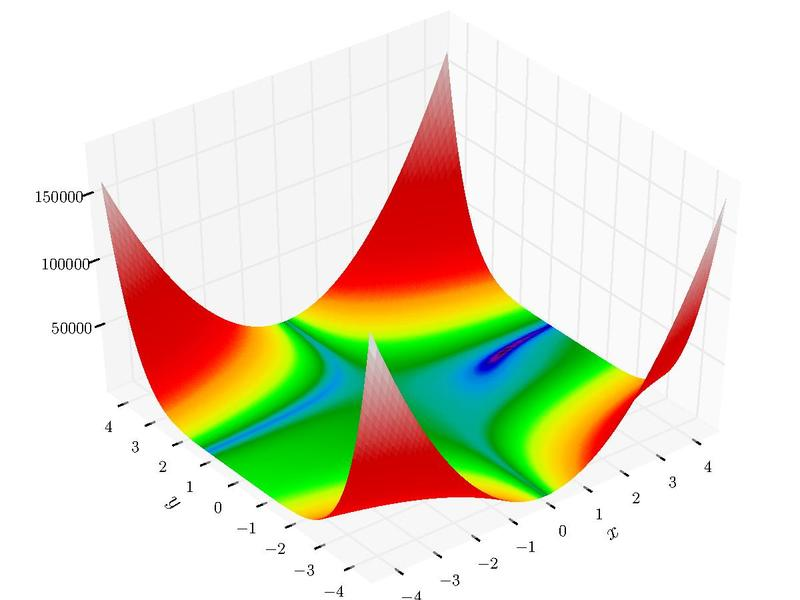
\includegraphics[width=35mm]{Beale} \\
(a) Rosenbrock's function & (b) Beale's function \\[6pt]
 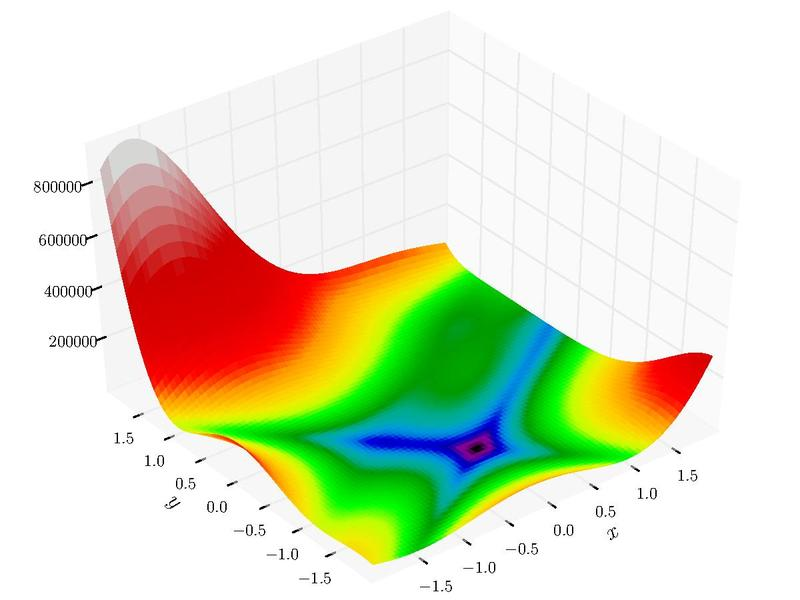
\includegraphics[width=35mm]{Goldstein_Price} &   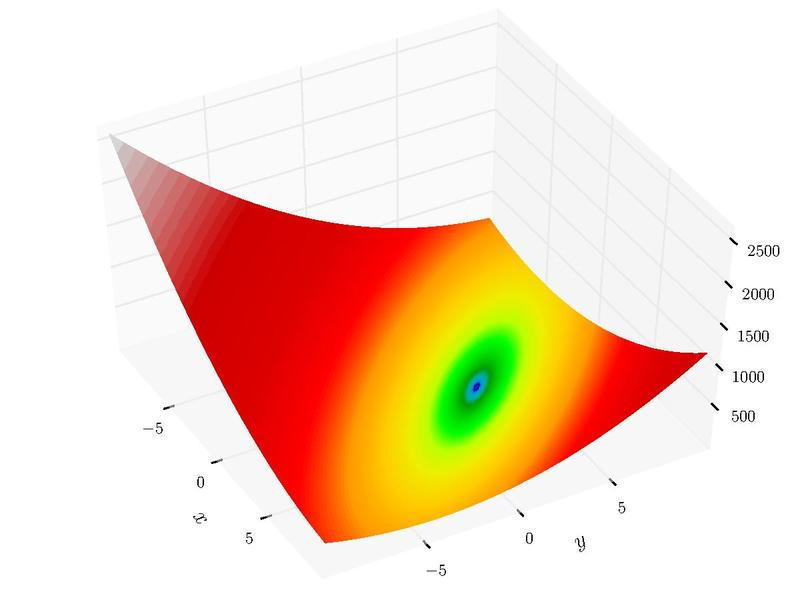
\includegraphics[width=35mm]{Booth} \\
(c) Goldstein-Price function & (d) Booth's function \\[6pt]
\end{tabular}
\caption{Examples of test functions for optimization.}
\label{testfunfig}
\end{figure}

\subsection{Non-differentiable/Non-deterministic Problems}
Following are some examples of NP-hard problems which tend to be non-deterministic and may be solved by MCMC methods.

\begin{itemize}
	\item{\textbf{The travelling salesman problem (TSP)}: It asks the following question: "Given a list of cities and the distances between each pair of cities, what is the shortest possible route that visits each city and returns to the origin city?" It is an NP-hard problem in combinatorial optimization \cite{b2}.}
	
	\item{\textbf{The closest string}: It is an NP-hard computational problem in theoretical computer science, which tries to find the geometrical center of a set of input strings. More formally, given $n$ length-$m$ strings $s1, s2, ..., sn$, the closest string problem seeks for a new length-$m$ string $s$ such that $d(s,si) ≤ k$ for all $i$, where $d$ denotes the Hamming distance, and where $k$ is as small as possible \cite{b4}.}

	\item{\textbf{The nurse scheduling problem (NSP)}: Also called the nurse rostering problem (NRP), it is the operations research problem of finding an optimal way to assign nurses to shifts, typically with a set of hard constraints which all valid solutions must follow, and a set of soft constraints which define the relative quality of valid solutions \cite{b5}.}
\end{itemize}

\section{Validation Metrics}
For either class of problems, I will evaluate the following metrics:
\begin{itemize}
	\item{\textbf{Robustness}: Convergence for different random initializations- can be evaluated for both deterministic and non-deterministic problems.}

	\item{\textbf{Efficiency}: Required memory and number of function evaluations- can be evaluated for either type of problems.}

	\item{\textbf{Accuracy}: For deterministic problems as well as low-dimensional non-deterministic problems, it is feasible to determine the optimal solution and check the accuracy in terms of mean squared error of the proposed solution. However, when the non-deterministic problems increase in dimension, determining the optimal solution becomes hard (hence they are known as NP-hard problems)}
\end{itemize}

\begin{thebibliography}{00}
\bibitem{b1} A. Bock, E. Grant, J. Konemann, and L. Sanita, “The School Bus Problem on Trees,” p. 10. \href{https://www.math.uwaterloo.ca/~jochen/docs/sbp.pdf}{link}
\bibitem{b2} “Travelling salesman problem,” Wikipedia. 16-Nov-2018. \href{https://en.wikipedia.org/w/index.php?title=Travelling_salesman_problem&oldid=869096463}{link}
\bibitem{b3} “Test functions for optimization,” Wikipedia. 22-Oct-2018. \href{https://en.wikipedia.org/wiki/Test_functions_for_optimization}{link}
\bibitem{b4} “Closest string,” Wikipedia. 09-Jun-2018. \href{https://en.wikipedia.org/wiki/Closest_string}{link}
\bibitem{b5} “Nurse scheduling problem,” Wikipedia. 21-Aug-2018. \href{https://en.wikipedia.org/wiki/Nurse_scheduling_problem}{link}
\bibitem{b6} M. Herman, “Simulated Annealing \& the Metropolis Algorithm: A Parameter Search Method for Models of Arbitrary Complexity,” p. 14. \href{https://pdfs.semanticscholar.org/3eea/67240fb0c2ec4f9ed5c61706c51dc770e102.pdf}{link}
\bibitem{b7} S. Towers, “Markov Chain Monte Carlo parameter optimization method | Polymatheia.” \href{http://sherrytowers.com/2014/07/15/markov-chain-monte-carlo-parameter-optimization-method/}{link}
\bibitem{b8} D. P. Kroese, T. Taimre, and Z. I. Botev, Handbook of Monte Carlo Methods. John Wiley \& Sons, 2013. \href{https://books.google.com/books?hl=en&lr=&id=Trj9HQ7G8TUC&oi=fnd&pg=PA1&ots=1EUdKeX7EE&sig=KU85plZUZghrbRSwrvlxZc6MHIg#v=onepage&q=441&f=false}{link}
\end{thebibliography}

\end{document}
